\section{Testing the basic economics \label{sec:frameworktestingbasicecons}}

This section demonstrates that the model framework successfully replicates what is known about the basic micro-economic ideas outlined in chapter \ref{chapter:location}. In doing so, it also picks out where there are problems and issues that need addressing.

\cmt{problems and issues need addressing... where?}

Problems: list here to write up -

Firms' DMR: cobb douglas means they can't - unless something like space costs are externalised. But then note, no longer a 'general' picture because some value must not enter into the picture. But it would let firms optimise...

%%%%%%%%%%%%%%%%%%%%
% PARTIAL VS GENERAL
%%%%%%%%%%%%%%%%%%%%
\subsection{Partial versus general analysis \label{sec:partialvsgeneral}}

\cmt{partial vs general: will this have been discussed in chapter 2 or 3? Discussing now in rel2 framework. I think somewhere around Fowler and equilibrium would be the best spot.}

Section x explained that a `general' analysis aims to include all factors affecting economic outcomes, because the full set of inter-relations may lead to very different outcomes from just looking at a partial picture. However, it was also argued [Isard etc] that such general analyses are made even more complex when space and agents become involved. Coordination issues abound, and space itself does away with the indispensable simplifying assumption of a single clearing market. This section goes into more depth, explaining exactly what this means for the modelling choices made in the thesis.

Of most importance is the fact that many partial models are used. This means fixing the majority of the model parameters to focus on one particular feature of interest. This makes for very different models. Consider the type of model Fowler presents (see section x): a number of Firms and People attempt to optimise revenue and utility respectively. Firms have economies of scale, wages are paid and goods have a cost. Both wages and good cost are set by `the market', which for an agent model must come about through either distributed decision-making, or otherwise some artificial construct to circumvent the coordination problem, like an auctioneer or, for the labour market, an assumption of collective bargaining. [Marc Oeffner]

%Taken from field diary, 'problems for later'. This is probably better for the intro.
To what extent do these coordination problems need solving before a full picture of spatial economics can be formed? Can these coordination issues be avoided by looking instead at partial analyses, while still saying something useful about spatial economics? Or does the coordination problems need solving before this can be known?

The model setups used for doing the basic checks below remain mostly the same. All People get a fixed wage (or a wage determined by the model); this means the overall level of demand is set exogenously. Firms' stock levels do not change: stock is always available to meet demand. All Firms have to do then, is maximise revenue by attempting to capture as much demand as they can. Aside from these two key features, others do vary. Firms may be mobile, optimising their location, while People remain immobile, and vice versa. Space cost changes are introduced through Goods' delivery cost.

I need to come back and summarise the setup for these tests.

\subsection{Coordination versus stochastics}

For many of the partial models, no real interaction is taking place between actors. Where People are deciding on location, if wages and prices are fixed, stock is unlimited and no density costs are incurred, each makes decisions entirely independently of the others. As a result, there is no difference between running a model with one actor a hundred times, or a hundred actors once. There is, however, a reason for running a multi-actor model in this situation: it allows for a quick understanding of the outcome of the underlying stochastic process. Outcomes are similar to entropy models \fixref{Wilson 1970, 'entropy in regional and urban modelling', from Haggett p.40}

Problem for me: I want to argue the following: The fact that one run with many actors is the same as many single-actor runs means that ,by using many, it is possible to get a very quick overview of the statistical outcomes for a particular setup.

However, I can't really argue that because there are no actual stats there. How to describe this? What is it?

This is not the case when Firms are making choices, as they do compete over the same total level of potential revenue.

%%%%%%%%%%%%%%%%%%%%%%
% CHECKING UTILITY
%%%%%%%%%%%%%%%%%%%%%%
\subsection{Checking utility \label{sec:checkutility}}

The first thing to do is to show how that actors' utility works as it should. 

The utility functions used as the basis for actors' demand all share certain common features and can be related to each other. 

%%%%%%%%%%%%%%%%%%%%%%
% COBB DOUGLAS
%%%%%%%%%%%%%%%%%%%%%%
\subsubsection{Cobb Douglas}

Actors with a Cobb Douglas utility function \eqref{eq:-3} want to buy a mix of two goods $F$ and $M$, where $p_F$ and $p_M$ are the price of $F$ and $M$ respectively. The constrained optima are as follows:
\cmt{this repeats equations from 'are black boxes teleological.' Probably need to pick one place for them.}

\begin{equation}
F=\frac{\delta Y}{p_F}\label{eq:optCDF}
%M=\frac{Y(1-\delta)}{p_{M}}-\delta\gamma\label{eq:engelpriceoptM}
\end{equation}
 
\begin{equation}
M=\frac{(1-\delta) Y}{p_M}\label{eq:optCDM}
%F=\frac{\delta Y-Y+\delta\gamma p_{M}}{p_{F}}\label{eq:engelpriceoptF}
\end{equation}

A key feature of the constrained Cobb Douglas is that the optimum for each good is independent of the other: it is dependent only on the price of that good, as well as the overall budget. Any change in the cost of one good, therefore, should not affect demand for the other. The flipside of this is that, because demand for the two goods is completely independent, the total revenue flowing from demand for each cannot change. Because of this, the Cobb Douglas share parameter $\delta$ exactly describes the income for each sector producing $F$ and $M$. Price-setting does not affect the income of the seller at all: each always gets exactly a $\delta$ share. In the \gls{coremodel}, this feature of the Cobb Douglas is useful, since it rules out any elasticity between the two sectors of manufacturing and food, keeping the analysis much simpler.

The independence of the two sectors in the Cobb Douglas also has a spatial consequence. In a situation where only two firms exist and space costs are internal to them, each producing one of $F$ and $M$, they can gain nothing by changing their location: their income will stay precisely the same. In this two-firm situation, this robs them of any meaningful action - a point to be returned to shortly.

\begin{figure}%
\centering
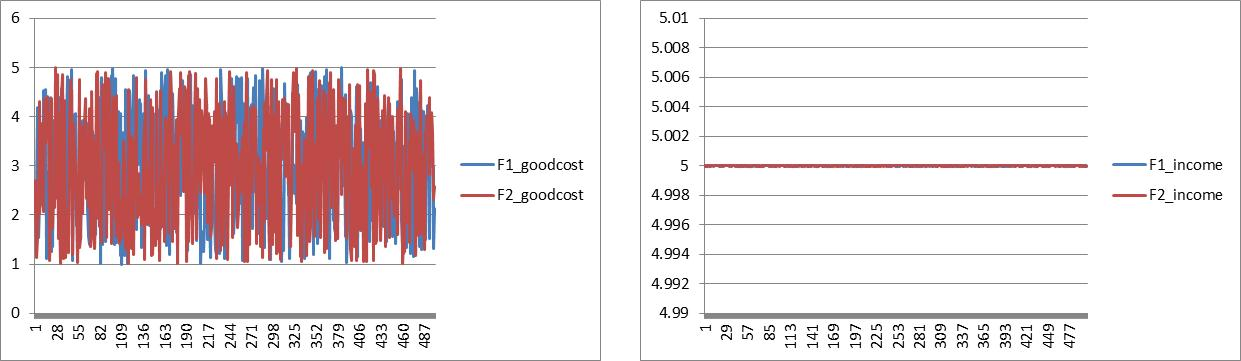
\includegraphics[width=0.85\columnwidth]{ChapterFramework/figures/CD_2firm_randomPricing}%
\caption{Two firms, Actors with Cobb Douglas utility, both firms randomising their price. First graph shows randomised price, second shoes income for the two firms.}%
\label{fig:CD_2firm_randomPricing}%
\end{figure}

Figure \ref{fig:CD_2firm_randomPricing} shows data from an agent model run where two firms set random prices for $F$ and $M$. It can be seen that both firm's income levels stay the same regardless of price. Price elasticity of demand, then, is unit elastic: any change in price is matched by a change in demand that keeps revenue levels static. This is as should be expected from Cobb Douglas utility. 

\begin{figure}%
\centering
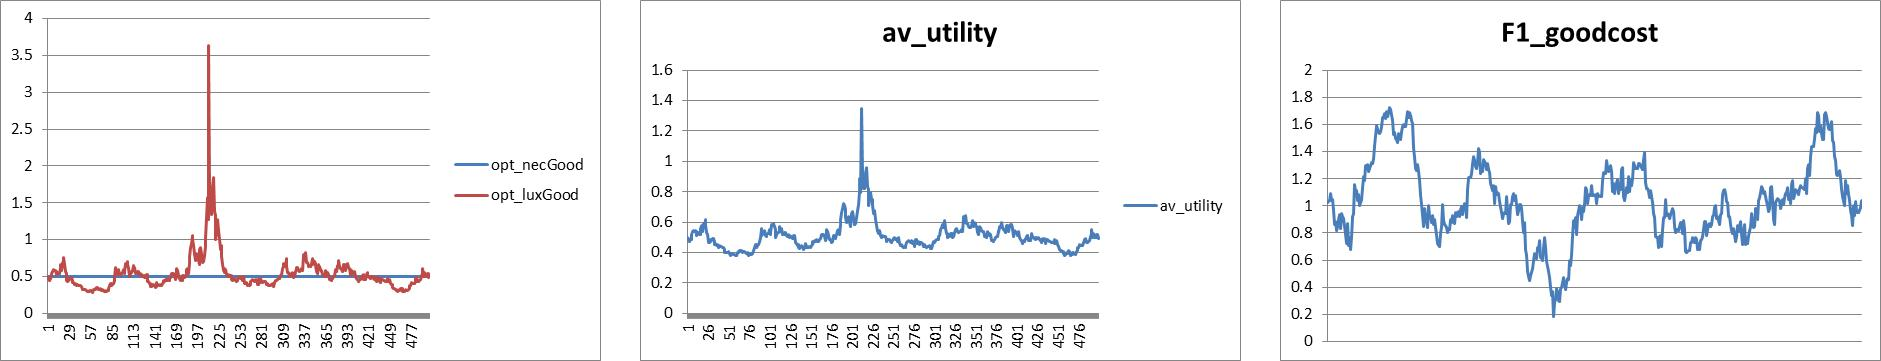
\includegraphics[width=0.85\columnwidth]{ChapterFramework/figures/CD_1fixed}%
\caption{Two firms, Actors with Cobb Douglas utility, one firm's price fixed.}%
\label{fig:CD_1fixed}%
\end{figure}

Figure \ref{fig:CD_1fixed} makes the same point in a different way: it shows the outcome when one firm's prices are fixed while the other attempts to find a revenue-maximising price. As mentioned above, this fails because they can affect no change on their revenue in this situation. For the fixed-price firm, actors consume a constant amount - and that is not altered by changes in the price of the other good. This shows that actors' demand for each is independent of the other. 

What else to say about the Cobb Douglas? Come back and stick in an example of externalities for space costs, problems for 'general' analysis.

--
Next: point of Engel function - compare to CES, where changing space costs makes no difference to spatial outcomes, just has entirely predictable, aspatial impact on overall utility. Who cares about that?


%%%%%%%%%%%%%%%%%%%%%%
% CES
%%%%%%%%%%%%%%%%%%%%%%
\subsubsection{CES}

Like the Cobb Douglas, the Constant Elasticity of Substitution function sets up a situation where all goods of equal price enter into utility equally, regardless of the level of income. Spatially, one of the consequences of this is that the choices facing actors actually do not change as costs increase. Utility may drop, but discrete decisions about which firm to work for will remain the same, since the reasons behind those choices cannot change. 

\subsubsection{Engel function}

The Engel function breaks with the previous two utility functions: changes in costs \emph{do} affect actors' choices, and the level for each consumed good. Firstly, figure \ref{fig:engeltest_income1to2} shows that actors in the model framework will reproduce the Engel function dynamic discussed in section \ref{sec:utilityengelslaw}. Note, however, that it does not perfectly match the analytic result: the utility algorithm never quite manages a perfect match. One result of this is that where usually no demand for the luxury good should be present, there is a slight amount. \cmt{Imperfections in Engel function. Is that still the case now? Need to check - algorithm may have massively improved.}

\begin{figure}%
\centering
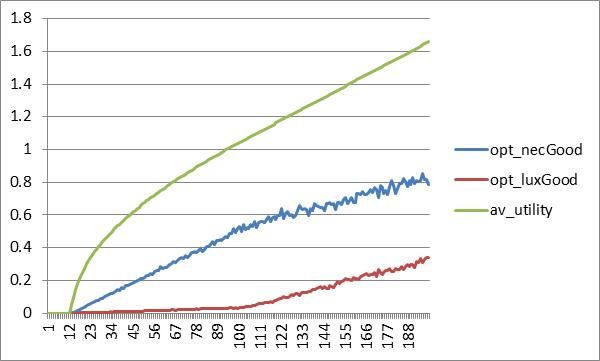
\includegraphics[width=0.4\columnwidth]{ChapterFramework/figures/engeltest_income1to2}%
\caption{Testing the Engel utility function: $\gamma = 1$, wage level changed from 1 to 2.}%
\label{fig:engeltest_income1to2}%
\end{figure}

Actors do replicate the most important feature of the Engel function: when incomes are low (below the level set by $\gamma$, given unit prices), they demand only the necessity good (plus some small extra amounts of luxury good resulting from small random fluctuations in the optimisation routine).

%%%%%%%%%%%%%%%%%%%%%%%%
% BASIC SPATIAL OUTCOMES
%%%%%%%%%%%%%%%%%%%%%%%%
\section{Basic spatial outcomes from the basic economics}

\cmt{Yes, that needs a better title. Let's just get writing.}

Within the limitations of partial analyses, agent-based actors do still find optimal spatial outcomes of interest. This section outlines the most interesting from within the model framework. 

Cost structure for homothetic versus non-homothetic functions has a different impact.

%%%%%%%%%%%%%%%%%%%%%%%%
% BLACK HOLE
%%%%%%%%%%%%%%%%%%%%%%%%
\subsection{The obvious black hole outcome \label{sec:blackholemodel}}

Space imposes costs and, like any other cost, actors will minimise it if they can. The most obvious spatial outcome is that all actors will simply remove those costs, collapsing to a point in the process, unless other forces mitigate against this. Such forces exist; one outcome of using them is discussed in the next section. But without them, does the model reproduce the basic `black hole' finding? Here, with all other costs fixed, Firms and People are allowed to find their preferred location using the methods described above - People comparing different Bundle locations and Firms using a feedback that crawls towards revenue-improving locations.

\begin{figure}
  \centering
 %\subfloat[A gull]{\label{fig:gull}\includegraphics[width=0.3\textwidth]{gull}}                
  %\subfloat[A tiger]{\label{fig:tiger}\includegraphics[width=0.3\textwidth]{tiger}}
  \hspace{0.2}     
  \subfloat[People]
  {\label{fig:bhg2}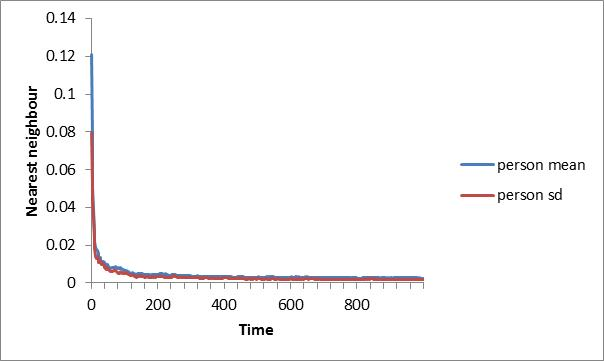
\includegraphics[width=0.4\textwidth]{ChapterFramework/figures/mnnd_blackhole_manyruns1}}
  \hspace{0.2}  
  \subfloat[Firms]{\label{fig:bhg3}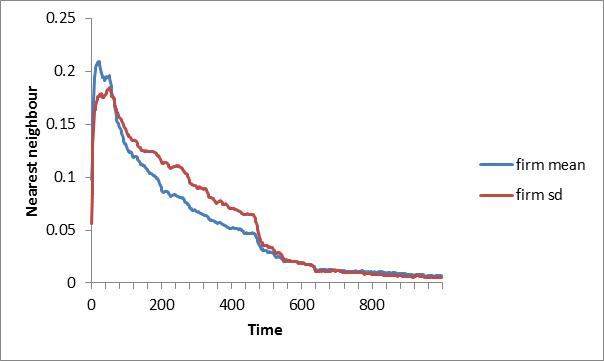
\includegraphics[width=0.4\textwidth]{ChapterFramework/figures/mnnd_blackhole_manyruns2}}
  \caption{Means and standard deviations of nearest neighbour distance, randomised starting locations, averaged from 20 model runs.}
  \label{fig:blackholegraphs}
\end{figure}

\cmt{MNND: meaning of SD is different in spatial context. These are perhaps placeholders, while we get text done, then work out what needs more detail and of what sort.}
%Data: location1/data/nearestneigh20runs

Figure \ref{fig:blackholegraphs} shows the outcome of this model run over a thousand days for twenty People and four Firms. The model was run twenty times with different random starting conditions; the data shows the average outcome. All actors converge on a point, incrementally seeking positions closer to each other to reduce space costs or, in Firms' case, increase revenue. People quickly converge, while Firms take much longer: this reflects the fact that Firms must use a feedback that cannot always be relied upon - section x discusses this point in detail. \cmt{Video x in location y, a typical run showing how actors decide, gotta work out where that's going.} Ultimately, all actors do reduce their space cost as close to zero as they can.
\cmt{Question: basic black hole outcome. Are competition effects having an impact on completely stopping this collapse?}
\cmt{Should also write up: `lock-in' effect when many actors are on same spot; each reinforces the location of the other. Once formed, the exact location of a black hole point will not change/drift unless perturbed.}

%%%%%%%%%%%%%%%%%%%%%%%%%%%%%%%%
% CONTINUOUS SPATIAL EQUILIBRIUM
%%%%%%%%%%%%%%%%%%%%%%%%%%%%%%%%
\subsection{Spatial equilibrium}

Density cost is used as a proxy to reflect generic `land costs', covering both the effect of rent and congestion (see section x.) 

As discussed in section x, a very simple way of avoiding spatial `black holes' where all actors collapse into a point is to impose a density cost. Once again, this is only a partial solution: real land use is subject to the law of supply and demand where actors bid over prices. A density cost can only be a loose proxy. However, it can be used with all the same caveats that attach to any `partial' solution that imposes a fixed cost. 

\cmt{black holes: model tested above, but not discussed anywhere yet. I think I have mentioned it as the spatial impossibility theorem... Also, density cost isn't quite a fixed cost is it? It's a proxy for rent and congestion, where the market part of the process is replaced by a stand-in that mimics its effect.}

This section explains the use of the density cost in full. That is done here so it can be seen in use in two model situations, one that replicates the standard utility-equilibrium finding from urban economics, another that breaks it, where actors utility does not equilibriate.
\cmt{`standard utility-equilibrium finding from urban economics' where to x-ref this to?}

%The model setup is the same as for testing the `black hole' outcome above, except for the imposition of a density cost, and an increase in the number of People to a thousand in order to allow a clear picture of the spatial outcome. (Numbers do not directly affect the actual density cost, since it is calibrated to the number of people in any particular model run.)

%NEEDS MOVING TO FRAMEWORK CHAPTER
\subsection{The setup for density cost \label{sec:densitycostsetup}}

Density cost uses three parameters: a radius around each Actor incurring the cost, the cost itself, defined as a value between zero and one, and a third value, `found density', which calculates density of actors within the radius, also returning a value between zero and one (this method will be described in detail next). This is imposed as a `tax' directly on People's wage. Let $dc$ be density cost -

\begin{equation}
dc = cost * found\ density
\label{eq:densitycost}
\end{equation}

The found value of $dc$ is then subtracted from the wage. Note that the density cost is independent of the wage, so it will become proportionately smaller as wages rise. The main method for calculating `found density' is as follows, where `me' is the Person doing the calculation:

\begin{itemize}
	\item Using the density cost radius, normalise all Actors' distance from me to between one and zero, where one is the same location as me, and zero is on or beyond the radius.
	\item Sum these normalised distances, then divide by the total number of Actors.
\end{itemize}

The resulting value is one if all Actors are exactly in the same location as `me', zero if none are within the density cost radius, and between zero and one otherwise. 
\cmt{Density cost: pretty sure this is the same method (or variant of) used for kernel density estimation. (kernel just means radius, afaik.)}


\subsubsection{Basic model test of density cost; effect compared to black hole model}

What impact does a density cost have on model outcome? To test this, the setup from the `black hole' model is used, with two changes. First, Firm location is fixed at a centre-point. Since the feature of interest is density cost, it is assumed that firms have found their way to a central point as they do in section \ref{sec:blackholemodel} above. (Note that, while in the `black hole' model test, Firms do not quite centre perfectly, this small difference from exact centring has no material impact on the test here, so it is easier to assume that centring has taken place.) Second, the number of People is increased in order to allow a clear picture of the spatial outcome.

\cmt{I'd written: `Population size does not directly affect the actual density cost, since it is calibrated to the number of people in any particular model run, but it does affect the exact morphology of the spatial pattern that results.' But I think I need to explain that above in the density cost description, not here. Tricky: in some situations, actor number will make a difference, e.g. for work distance of 1 day, if that's a hard limit for all actors, then they'll need to cram closer together if there's more.}

A test model was run for 1200 days with 1000 People. Over that run, twenty-three values for good space-cost were exogenously changed, ranging from 500 to 0.01. These values were chosen specifically to illustrate discrete changes in the spatial outcome. The visual result for six of these are shown in figure \ref{fig:densityCostChange1}. Green squares are People, grey circles indicate the density cost radius for each Person. The model starts from something close to the `black hole' model where good space-costs are high enough to make density cost relatively unimportant. As good space-costs drop, People self-organise into concentric rings initially, before costs decrease enough for them to find interstitial points that minimise density costs, resulting in the hexagonal pattern observed. 

\begin{figure}
  \centering
  \subfloat[500]  {\label{fig:dc1}
\includegraphics[width=0.3\textwidth]{ChapterFramework/figures/densitycost1/sequence/torus-0026_FirmDelCost-500}}
  \hspace{0.1}    \subfloat[5]{\label{fig:dc2}
\includegraphics[width=0.3\textwidth]{ChapterFramework/figures/densitycost1/sequence/torus-0301_FirmDelCost-5}}
  \hspace{0.1}    \subfloat[1]{\label{fig:dc3}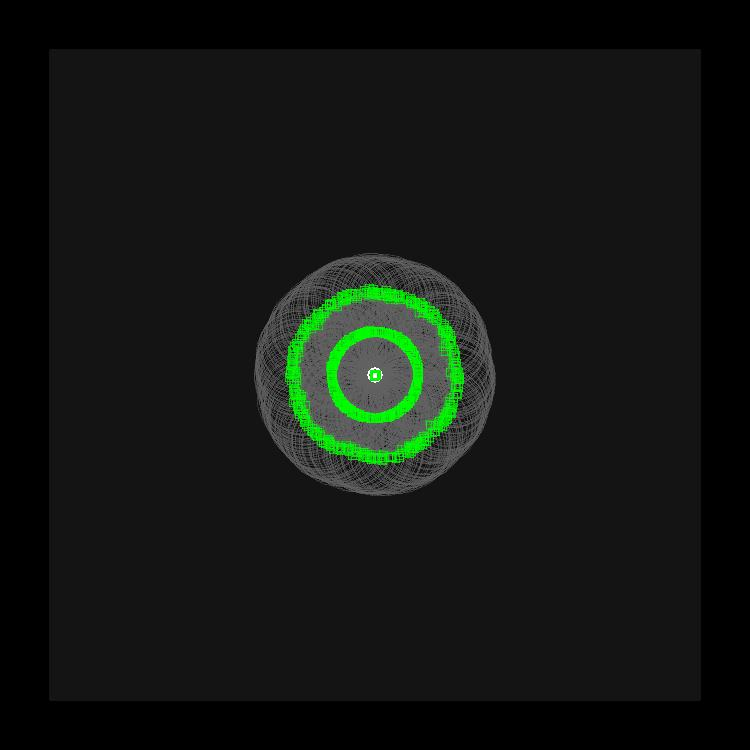
\includegraphics[width=0.3\textwidth]{ChapterFramework/figures/densitycost1/sequence/torus-0376_FirmDelCost-1}}
  \hspace{0.1}    \subfloat[0.5]{\label{fig:dc4}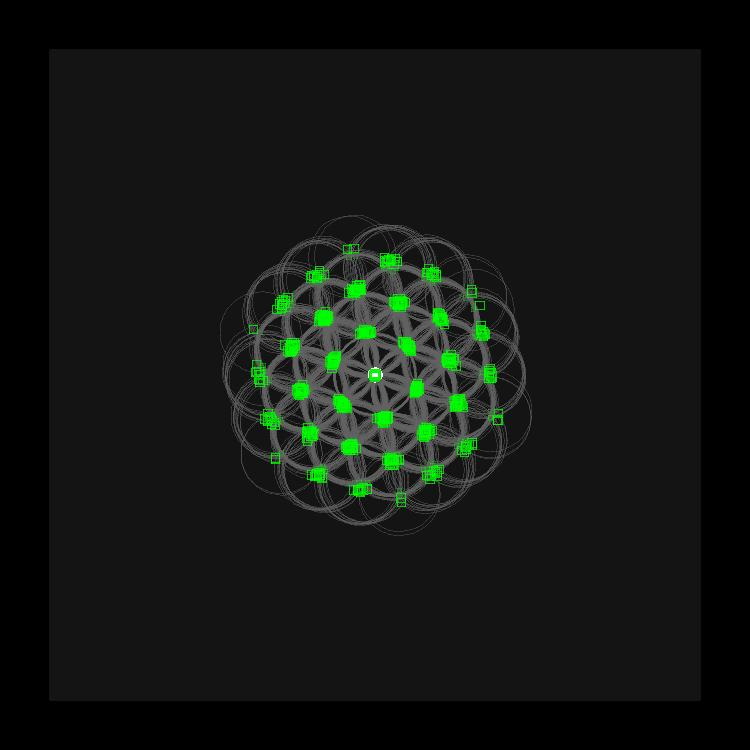
\includegraphics[width=0.3\textwidth]{ChapterFramework/figures/densitycost1/sequence/torus-0426_FirmDelCost-0-5}}
  \hspace{0.1}     \subfloat[0.125]{\label{fig:dc5}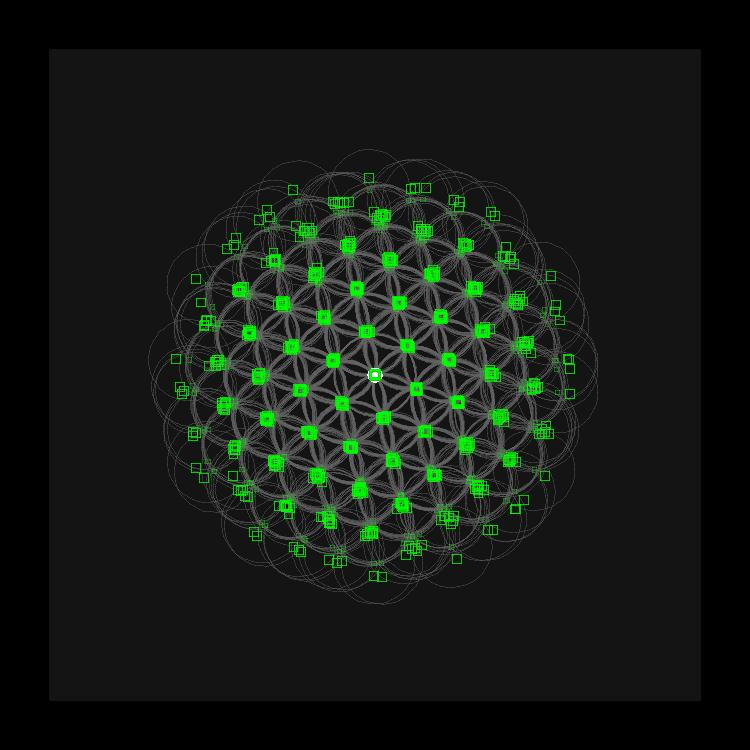
\includegraphics[width=0.3\textwidth]{ChapterFramework/figures/densitycost1/sequence/torus-0476_FirmDelCost-0-125}}
  \hspace{0.1}     \subfloat[0.05]{\label{fig:dc6}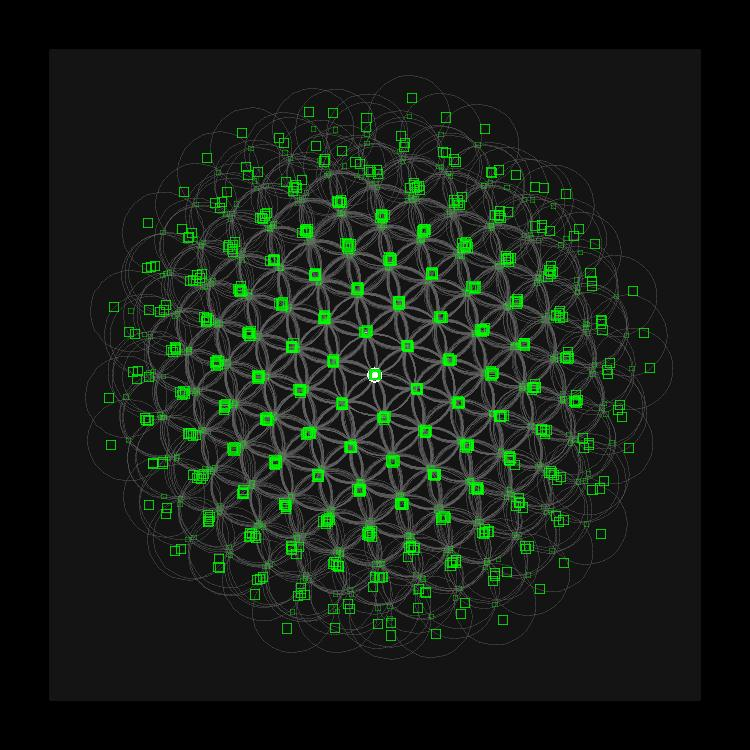
\includegraphics[width=0.3\textwidth]{ChapterFramework/figures/densitycost1/sequence/torus-0526_FirmDelCost-0-05}}
  \caption{Spatial equilibrium test. Visualisation of good space-cost changes interacting with density cost for six good space-cost values; spatial equilibrium outcome. 1200 days, 1000 People.}
  \label{fig:densityCostChange1}
\end{figure}

Figures \ref{fig:dc7} and \ref{fig:dc8} show data for mean utility and distance from the centre-point over the whole run. Each increase in mean utility is triggered by a decrease in good space-cost, and \ref{fig:dc8} illustrates that each of these leads to a larger spatial reach for all People. The important part of \ref{fig:dc7} is the standard deviation: it remains close to zero regardless of the space cost. Utility levels for all People quickly equalise. This is a spatial equilibrium outcome - all People are ending up with the same utility levels by self-organising in space. 
%For example, one Person moving out from the inner circle lowers the density cost there. For a given good space cost, this one move may be enough to equilibriate utility. If not, others will move out until that has happened.
%Perhaps explain that better!

\begin{figure}%
\centering
\subfloat[]
{\label{fig:dc7}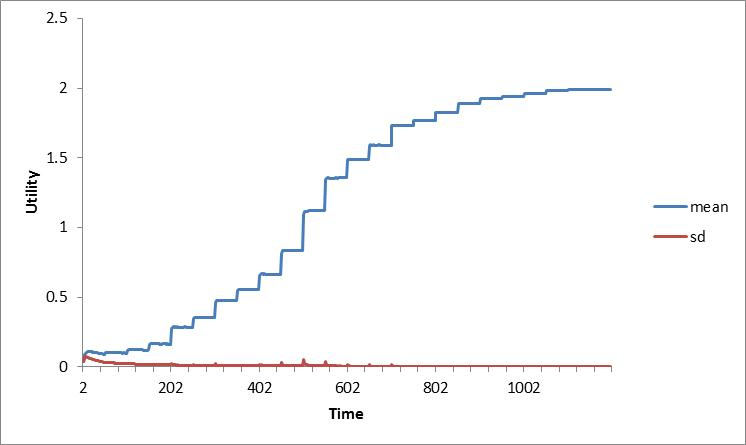
\includegraphics[width=0.4\columnwidth]{ChapterFramework/figures/densitycost1/densityseq_utiilty}}%
\hspace{0.2}  
\subfloat[]{\label{fig:dc8}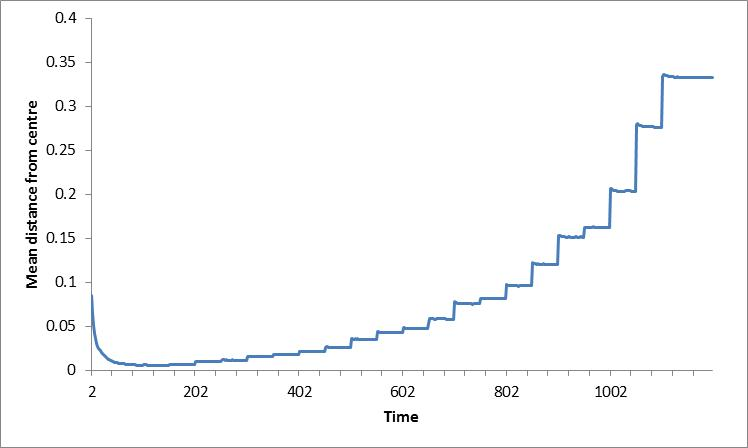
\includegraphics[width=0.4\textwidth]{ChapterFramework/figures/densitycost1/densityseq_meandistfromcentre}}
\caption{Spatial equilibrium test. Utility and mean distance from centre. Utility standard deviation shows equilibrium.}}%
\label{fig:spatialeq2}%
\end{figure}

This begs the question: why and how do they end up with the same level of utility? A fuller exploration of this question is discussed next; a descriptive answer will help set the context for that. In the model framework, People do only one thing: compare a range of options and choose the one that makes them better off. In moving, they are not aiming to improve matters for those in denser regions, but that is nevertheless what happens. They reduce density cost both for themselves and for others - but only when doing so allows them to be better off. The flipside is that they will only find moving makes them better off when their current density cost becomes too high, compared to other locations. This is, of course, a long way of saying that the system equilibriates. The value of the model is in confirming that this result is an inescapable consequence of many Actors pursuing their own interests.
%Again, rubbish last sentence!

\subsubsection{bits}

People are trading off two space costs: density and the cost of moving goods. For these model runs, the former is fixed. When good movement costs change, utility \emph{does} change, and for a period of time, it will vary - but People will self-organise their way back to an equilibrium of utility values. This is the situation illustrated in figures \ref{fig:dc1} to \ref{fig:dc6}. But is it possible to use the model to say more about the nature of this process? 

It is somewhat surprising that the density cost method produces a spatial equilibrium outcome. After all, no land rent mechanism is present - it is purely a weighted density cost of the sort used in kernel density calculations. So what can account for this? 
%And is it actually as surprising as all that?

%I want to end by confirming that this weighted density cost is (for the purposes here) a reasonable enough proxy for land rent costs that can produce good economic outcomes, without having to directly model land actors and landlords, as I was doing. 
%Also concluding: given some variable land cost, actors will generally equilibriate their utility. That said, of course, I haven't explained why that doesn't happen in backyard yet.
What all this means: Actors in a spatial equilibrium setting will produce an equilibriated `indifference map' showing where utility is equalised. This is an interactive process, distinct from a purely statistical outcome. A way to illustrate this is to move the two firms apart slightly. Since People have \gls{lov}, what will the `indifference map' look like?

Density cost is a `second nature' effect - it is entirely relative to the location of each Actor, not determined by absolute location. This might seem contrary to how actual land markets work: surely each parcel of land has a specific location? True, but the value of that land is not set, it is determined by demand. This helps explain how the density cost method manifests a spatial equilibrium outcome - but the model does this without having to assume exogenous rent levels that drop off from some central point.

Actors' ability to collectively produce a spatial equilibrium appears to be independent of the exact nature of the land cost involved. While different methods do produce different spatial morphologies, utility still equilibrates. Figure x compares three visualisations for three slightly different density cost calculating methods.

spatial interdependency crucial 





%%%%%%%%%%%%%%%%%%%%%%%%
% CES/SPACE BASICS
%%%%%%%%%%%%%%%%%%%%%%%%
\subsection{CES and continuous space}

In the fixed-model testing environment described above \cmt{define the fixed-model environment for testing the utility functions}, actors with \gls{lov} utility, having a guaranteed wage, need only to maximise utility given the space cost for each good. The basic spatial outcome is intuitive: the location actors find is central to a given cluster. However, an interesting discrete outcome arises as a result of the rapid drop-off of demand for any one good as costs increase.

\cmt{Need to explain: in CES, a linear range of prices leads to a non-linear demand pattern. E.g. if two goods, the double-price good has less than half demand.}


%%%%%%%%%%%%%%%%%%%%%%%%
% CES/SPACE BASICS
%%%%%%%%%%%%%%%%%%%%%%%%
\subsection{Engel Function and space}

For the Engel function, a change in costs can shift actors' optimal choice discretely. Actors find utility maximised by siting themselves next to whichever producer gives them the highest marginal utility. The principle is simple enough: if an actor has the option of siting themselves near one of two goods suppliers, and both have space costs, they will minimise the space cost for the one that benefits them the most. 

And now I need some diagrams.







%Question: how come backyard model has utility dropping off? Why no equilibrium there? Interesting question!

%%%%%%%%%%%%%%%%%%%%%%%%%%%%%
% CUTTINZ
%%%%%%%%%%%%%%%%%%%%%%%%%%%%%
\begin{comment}

Graphs for MNND distance. Currently using many-run averages...

\begin{figure}
  \centering
 %\subfloat[A gull]{\label{fig:gull}\includegraphics[width=0.3\textwidth]{gull}}                
  %\subfloat[A tiger]{\label{fig:tiger}\includegraphics[width=0.3\textwidth]{tiger}}
  \subfloat[All actors]
  {\label{fig:bhg1}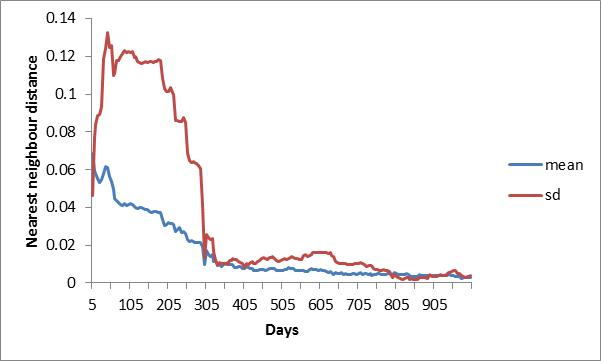
\includegraphics[width=0.4\textwidth]{ChapterFramework/figures/mnnd_blackholegraph1}}
  \hspace{0.2}     
  \subfloat[People]
  {\label{fig:bhg2}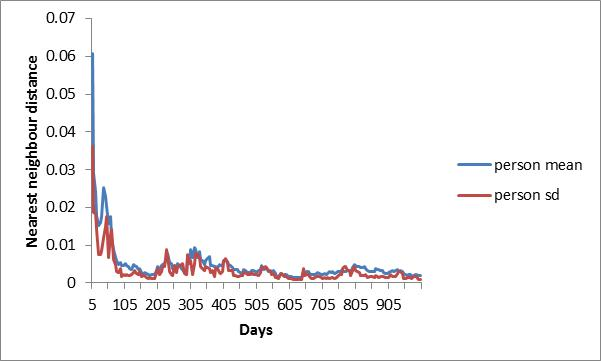
\includegraphics[width=0.4\textwidth]{ChapterFramework/figures/mnnd_blackholegraph2}}
  \hspace{0.2}  
  \subfloat[Firms]{\label{fig:bhg3}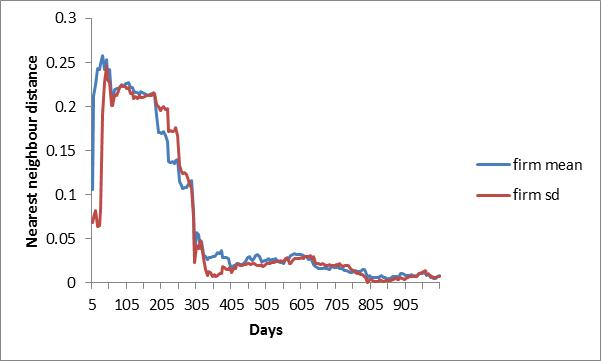
\includegraphics[width=0.4\textwidth]{ChapterFramework/figures/mnnd_blackholegraph3}}
  \caption{Mean and standard deviation of nearest neighbour distance, randomised starting locations}
  \label{fig:blackholegraphs}
\end{figure}
\end{comment}